\documentclass[../paper.tex]{subfiles}
\graphicspath{ {../images/} }

% Document
\begin{document}
    So, let's talk about the results we obtained.
    \subsection{CNN}
    We made two models, one makes use of pixel values while the other makes use of landmarks.
    Note that this is based on a reduced dataset, as we only have 6 letters.
    This is because of the hardware limitations, as we can't train effectively on a bigger dataset.
    \subsubsection{Pixel}
    The pixel model didn't perform as well as we hoped, because it makes use of the pixel values, it needs a lot of data to perform well.
    The model reaches an accuracy of 0.4 during training and stops learning quickly afterwards.
    We tried to fix this by adding more data, by augmentation, but this didn't help.
    \subsubsection{Landmarks}
    Landmarks performed better than the pixel model, as it only needs 21 landmarks to predict the letter.
    Not only that, the landmarks train based on position, so enviroment doesn't matter.
    The model during testing reaches an performance of 0.6667, whith a dataset of only 6 letters.
    \subsection{Graphs}
    We made a few graphs to show the performance of the models.
    \begin{figure}[h]
        \centering
        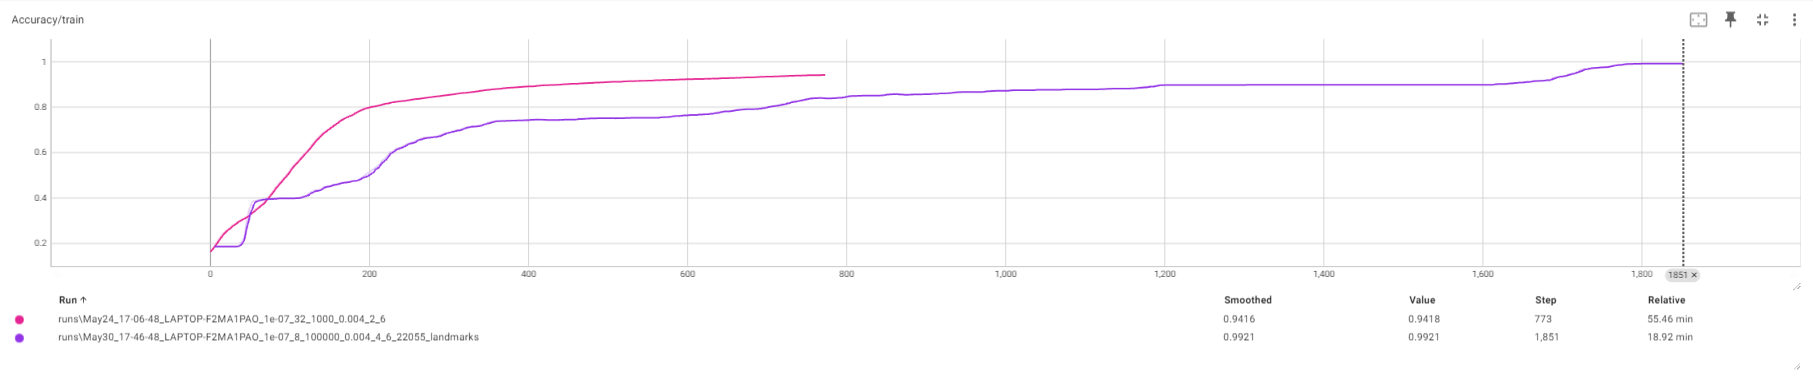
\includegraphics[width=\linewidth]{best_models}
        \caption{pixel vs landmarks}
        \label{fig:pixel_vs_landmarks}
    \end{figure}
    We can see how the training evolves over time. 
    The green line represents the pixel model, while the blue line represents the landmarks model.

    We can also look at the evolution of all models that we trained.
    \begin{figure}[h]
        \centering
        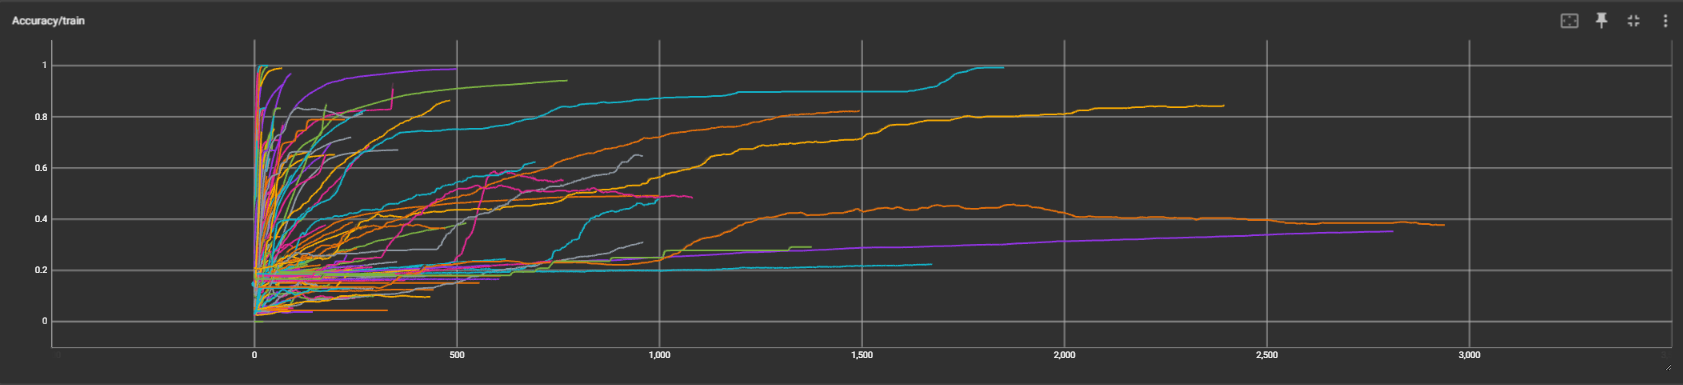
\includegraphics[width=\linewidth]{accuracy_graph_all}
        \caption{accuracy graph for all models}
        \label{fig:all_models}
    \end{figure}
    As you can see the figure \ref{fig:all_models}, we had struggles with many models, and eventually only one model out of many performed well.

\end{document}
